\documentclass[12pt,a4paper]{article}
\usepackage[a4paper,top=2cm,bottom=2cm,left=2.5cm,right=2cm]{geometry}
\usepackage{fontspec}
\setmainfont{Liberation Serif}
\setmonofont{Liberation Mono}
\usepackage[english]{babel}
\usepackage{graphicx}
\usepackage{amsmath}
\usepackage{array,tabularx,longtable}
\usepackage{caption}
\usepackage{enumitem}
\usepackage{setspace}
\usepackage{titlesec}
\usepackage{fvextra}
\PassOptionsToPackage{hyphens}{url}
\usepackage[hidelinks,hypertexnames=false]{hyperref}
\urlstyle{same}
% Personal details and report title.
\newcommand{\studentname}{Balan Gabriel}
\newcommand{\studentgroup}{FAF-241}
\newcommand{\supervisorname}{Maia Zaica}
\newcommand{\reporttopic}{Cryptanalysis of Monoalphabetic Ciphers}
\newcommand{\repositoryurl}{https://github.com/AverageCEnj0yer/Cryptography}

\hypersetup{pdftitle={Laboratory Work No. 2: Cryptanalysis of Monoalphabetic Ciphers},pdfauthor={Balan Gabriel}}
\setstretch{1.25}
\setlength{\parindent}{1.1cm}
\setlength{\parskip}{4pt}
\setlength{\emergencystretch}{2em}
\setcounter{tocdepth}{2}
\titleformat{\section}{\large\bfseries}{\thesection}{0.65em}{}
\titleformat{\subsection}{\normalsize\bfseries}{\thesubsection}{0.65em}{}
\captionsetup{font=small,labelfont=bf,skip=6pt,hypcap=false}
\newcolumntype{Y}{>{\raggedright\arraybackslash}X}
\setlist{itemsep=2pt,topsep=4pt}
\fvset{fontfamily=tt,fontsize=\footnotesize,baselinestretch=1,
  breaklines=true,breakanywhere=true}
\newcommand{\mapto}[2]{\texttt{#1}$\,\to\,$\texttt{#2}}
\newcommand{\sample}[1]{\VerbatimInput{data/#1}}
\begin{document}

% -----------------------------------------------------------------------------
% Cover page: the requested layout, adapted to Cryptography.
% -----------------------------------------------------------------------------
\begin{titlepage}
  \begin{center}
    \IfFileExists{assets/UTM_Logo_English.jpeg}{%
      
\includegraphics[width=3.4cm]{assets/UTM_Logo_English.jpeg}\par
    }{%
      \fbox{\parbox[c][1.7cm][c]{3.4cm}{\centering\textbf{UTM LOGO}}}\par
    }
    \vspace{0.25cm}
    {\bfseries\fontsize{14}{17}\selectfont
      MINISTRY OF EDUCATION, CULTURE AND RESEARCH\par
      OF THE REPUBLIC OF MOLDOVA\par
      Technical University of Moldova\par
      Faculty of Computers, Informatics and Microelectronics\par
      Department of Software Engineering and Automation\par
    }
    \vspace{1.4cm}
    {\bfseries\fontsize{16}{19}\selectfont \studentname\ \studentgroup\par}
    \vspace{1.5cm}
    {\bfseries\fontsize{36}{40}\selectfont Report\par}
    \vspace{0.2cm}
    {\itshape\fontsize{20}{24}\selectfont Laboratory Work No. 2\par}
    {\bfseries\itshape\fontsize{20}{24}\selectfont Cryptography\par}
    \vspace{0.8cm}
    {\fontsize{20}{24}\selectfont Topic: \reporttopic\par}
  \end{center}
  \vfill
  \begin{flushright}
    {\fontsize{15}{18}\selectfont Checked by:}\par
    \textbf{\supervisorname}, \textit{university assistant}
  \end{flushright}
  \vfill
  \begin{center}
    {\bfseries\fontsize{14}{17}\selectfont Chișinău -- 2026}
  \end{center}
\end{titlepage}

\setstretch{1.15}
\setlength{\parskip}{3pt}
{\setstretch{1}\small\setlength{\parskip}{0pt}\tableofcontents}
\clearpage
\section{Objective and scope}
The aim of this laboratory was to recover an English plaintext encrypted with a monoalphabetic substitution cipher, without knowing the substitution key. The work was carried out manually using the Crypto Corner frequency-analysis activity \cite{tool}. It was a cryptanalysis exercise, with no programming implementation required.

The solution combined letter frequencies with repeated words, common letter combinations, grammatical context, and consistency across the passage. The working record contains 19 deduction steps; several steps establish more than one letter pair. This report follows that order and illustrates how successive substitutions make the message readable. The ciphertext and the final literal decryption are included in the appendices.

\section{Theoretical background}
\subsection{Monoalphabetic substitution and its weakness}
A monoalphabetic substitution replaces each plaintext letter with a fixed ciphertext letter throughout a message. For an alphabet $\mathcal{A}$ of 26 English letters, let $\pi$ be a permutation of that alphabet. Encryption and decryption are
\begin{equation}
  c_i=\pi(p_i),\qquad p_i=\pi^{-1}(c_i).
\end{equation}
A general substitution has $26!\approx4.03\times10^{26}$ possible keys. This is far larger than the 25 nonzero shifts of the English Caesar cipher, but the size of the key space does not remove statistical structure. Every occurrence of a plaintext letter receives the same replacement. Repeated letters, repeated words, and frequency patterns survive under different labels.

The analysis therefore targets language structure rather than trying every key. If a plaintext letter appears $n$ times, its ciphertext replacement also appears $n$ times. When spaces and punctuation are retained, as in this cryptogram, they provide additional clues about word lengths, sentence boundaries, and possessive forms.

\subsection{Letter-frequency analysis}
The course material explains that letters occur at different rates in natural languages \cite{handout}. For a ciphertext containing $N$ letters, the observed percentage of a symbol $c$ is
\begin{equation}
  f_C(c)=\frac{n_C(c)}{N}\times100\%,
\end{equation}
where $n_C(c)$ counts that symbol. Uppercase and lowercase forms are counted together. Spaces, punctuation, digits, and line breaks are excluded from $N$.

A sufficiently long ordinary passage often resembles the broad frequency profile of its language, although subject matter and writing style cause deviations. English is the relevant reference for this exercise. The Romanian frequencies in the handout illustrate the same language-dependent principle, but they are not the reference used to solve this English passage.

\begin{table}[htbp]
\centering
\caption{English reference frequencies from the supplied course material (percent)}
\label{tab:english}
\small
\begin{tabular}{rr@{\hspace{1.3cm}}rr}
\hline
Letter & Frequency & Letter & Frequency\\
\hline
A & 8.17 & N & 6.75\\
B & 1.49 & O & 7.51\\
C & 2.78 & P & 1.93\\
D & 4.25 & Q & 0.09\\
E & 12.70 & R & 5.99\\
F & 2.23 & S & 6.33\\
G & 2.01 & T & 9.06\\
H & 6.09 & U & 2.76\\
I & 6.97 & V & 0.98\\
J & 0.15 & W & 2.36\\
K & 0.77 & X & 0.15\\
L & 4.03 & Y & 1.97\\
M & 2.41 & Z & 0.07\\
\hline
\end{tabular}
\end{table}

The most frequent ciphertext symbol is a candidate for plaintext \texttt{e}, but this is a hypothesis, not a rule. Matching the sorted frequency lists mechanically can produce incorrect substitutions. A few likely pairs constrain the key; they do not uniquely establish the entire permutation. Each proposal must also fit words and remain consistent with previously accepted pairs.

\subsection{Word patterns, digraphs and trigraphs}
A digraph is a pair of letters and a trigraph is a group of three. The supplied material lists common English digraphs such as \texttt{TH}, \texttt{HE}, \texttt{AN}, \texttt{IN}, \texttt{ER}, \texttt{ON}, \texttt{RE}, and \texttt{ED}. Useful trigraphs include \texttt{THE}, \texttt{AND}, \texttt{THA}, \texttt{ENT}, \texttt{ION}, and \texttt{TIO}. A recurring pattern such as \texttt{tQe} can therefore suggest the word \texttt{the} and the pair \mapto{Q}{h}.

Other clues include the ordinary one-letter English words \texttt{a} and \texttt{i}, common doubled letters such as \texttt{ss}, \texttt{ee}, \texttt{tt}, \texttt{oo}, and \texttt{ff}, and word shapes that survive substitution. Once several letters are known, a pattern such as \texttt{teYt} strongly suggests \texttt{text}. Context then tests the proposal across all occurrences, rather than accepting it because it fits one location.

\subsection{Method and limitations}
The working method was to compare frequencies, propose a substitution, inspect the partially decoded passage, and accept or reconsider the proposal based on additional words. Each ciphertext letter must have one consistent plaintext value; two ciphertext letters cannot both represent the same plaintext letter under the assumed permutation.

Long messages usually provide more repeated evidence than short ones, but even a long passage can have unusual vocabulary. Proper names and missing spaces are especially poor starting points. Here, common words were solved first; names such as Khnumhotep became readable later. Human judgement guided this particular exercise. This does not imply that substitution ciphers cannot be attacked automatically; the report describes the manual method used in the laboratory.

\clearpage
\section{Frequency evidence and working method}
\subsection{The supplied cryptogram}
The supplied text contains \textbf{2,567 alphabetic characters} and uses \textbf{25 distinct ciphertext letters}. Ciphertext \texttt{M} is absent. Counting the supplied text reproduces every integer count in the frequency screenshot, providing a check that the report uses the same cryptogram as the exercise.

The activity on the \href{https://crypto.interactive-maths.com/frequency-analysis-breaking-the-code.html}{Crypto Corner website} supplied the frequency displays used during the exercise \cite{tool}. The four images below are the supplied laboratory screenshots. The tables show the ranked distributions; the charts show the same kind of information in alphabetic order. The letter substitutions and their justifications come from the student's working notes \cite{records}.

\begin{center}
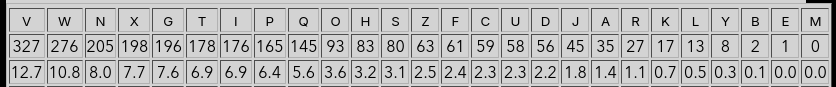
\includegraphics[width=\linewidth]{screenshots/frequency_table_encrypted.png}
\captionof{figure}{Ranked ciphertext frequencies: symbol, count, and rounded percentage}
\label{fig:cipher-table}
\end{center}

\begin{center}
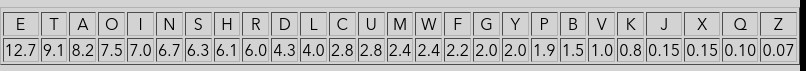
\includegraphics[width=\linewidth]{screenshots/frequency_table_english.png}
\captionof{figure}{Ranked English reference frequencies used for comparison}
\label{fig:english-table}
\end{center}

For example, ciphertext \texttt{V} occurs 327 times:
\begin{equation}
 f_C(\texttt{V})=\frac{327}{2567}\times100\%\approx12.74\%.
\end{equation}
This agrees closely with the English reference for \texttt{e}, approximately 12.7\%. Ciphertext \texttt{W} occurs 276 times, or approximately 10.75\%, and was proposed as \texttt{t}. The screenshot displays these as 12.7\% and 10.8\%. Its rounded reference figures may differ slightly from the two-decimal values in Table~\ref{tab:english}.

Frequency order alone is insufficient. The third most frequent ciphertext symbol is \texttt{N}, with 205 occurrences. A strict rank match would associate it with English \texttt{a}, whereas the readable word \texttt{to} establishes \mapto{N}{o}. Ciphertext \texttt{T}, only sixth in the observed ranking, is the actual replacement for \texttt{a}.

\subsection{Notation and consistency}
All mappings in the report run from ciphertext to plaintext: \mapto{V}{e} means that ciphertext \texttt{V} represents plaintext \texttt{e}. In intermediate extracts, unresolved ciphertext symbols are uppercase and recovered plaintext letters are lowercase. This convention avoids confusing an unsolved symbol with a letter that has already been identified.

The snapshots in Section~\ref{sec:progress} are reconstructed from the supplied ciphertext using the cumulative mappings in the recorded order. They are text illustrations, not additional screenshots of the website. This makes the progression internally consistent while preserving the original deduction logic.

\clearpage
\subsection{Visual comparison of the distributions}
\begin{center}
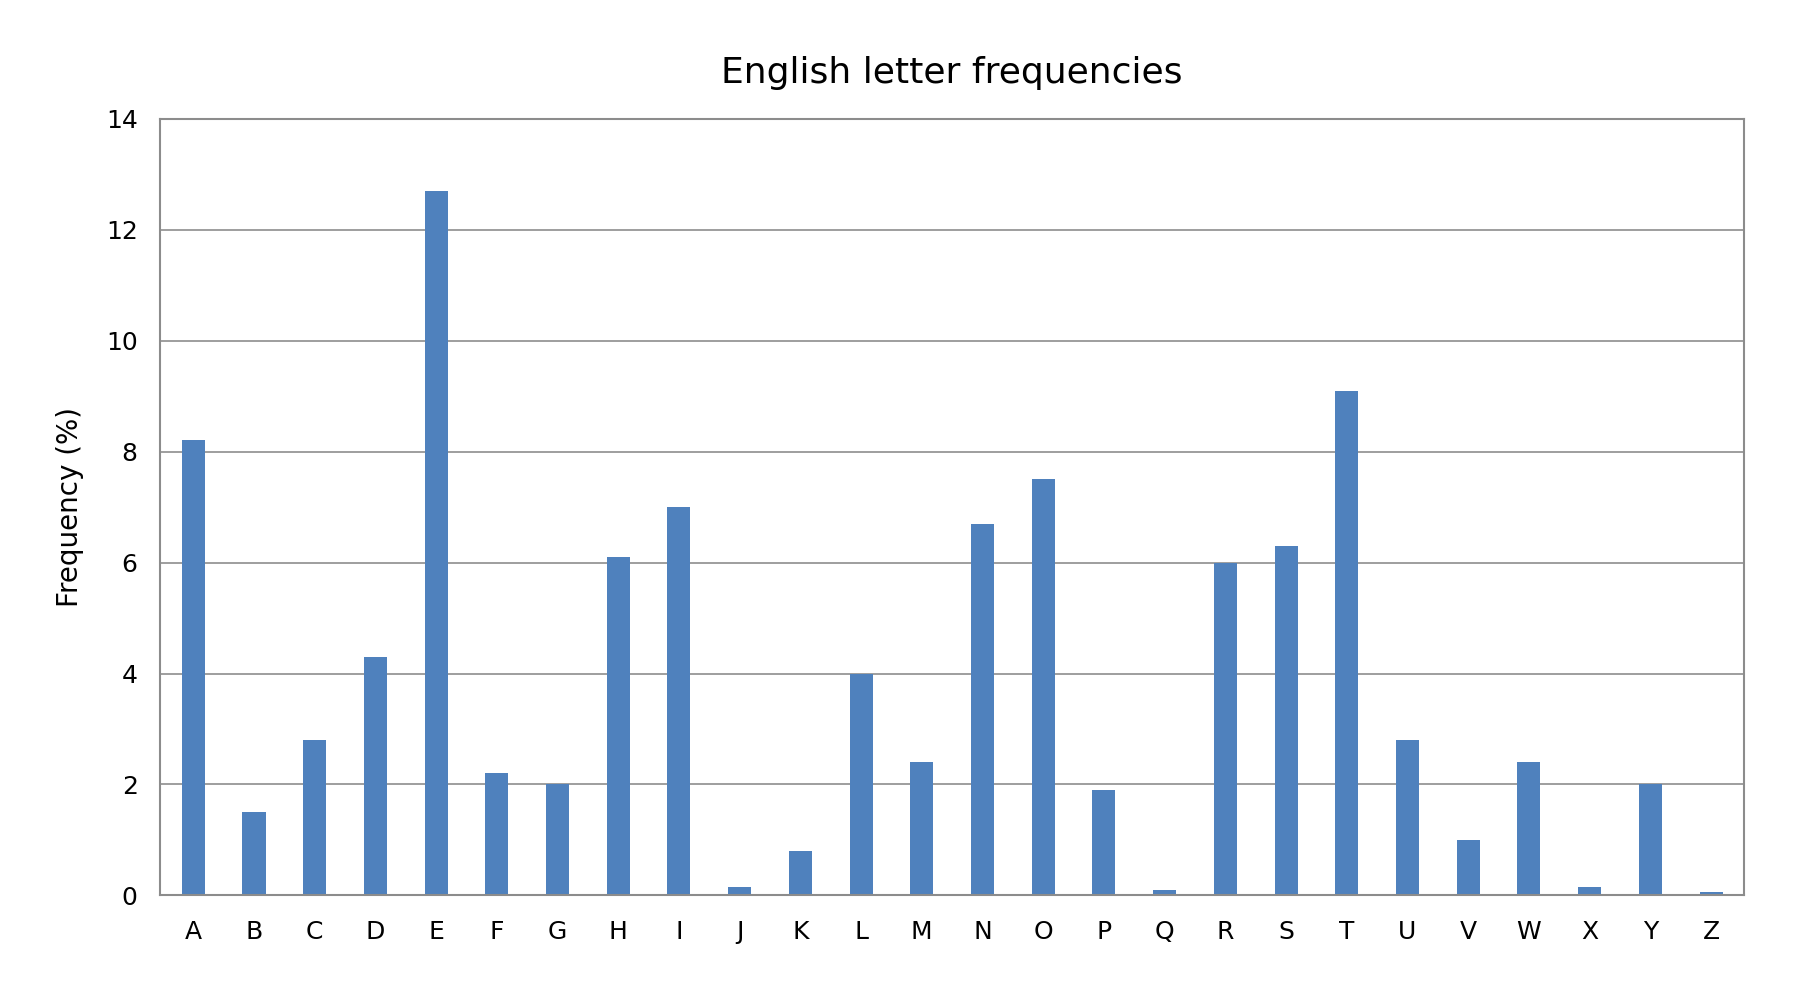
\includegraphics[width=0.94\linewidth]{screenshots/english_frequency_percentages.png}
\captionof{figure}{English reference profile: prominent peaks include E and T}
\label{fig:english-chart}
\end{center}

\begin{center}
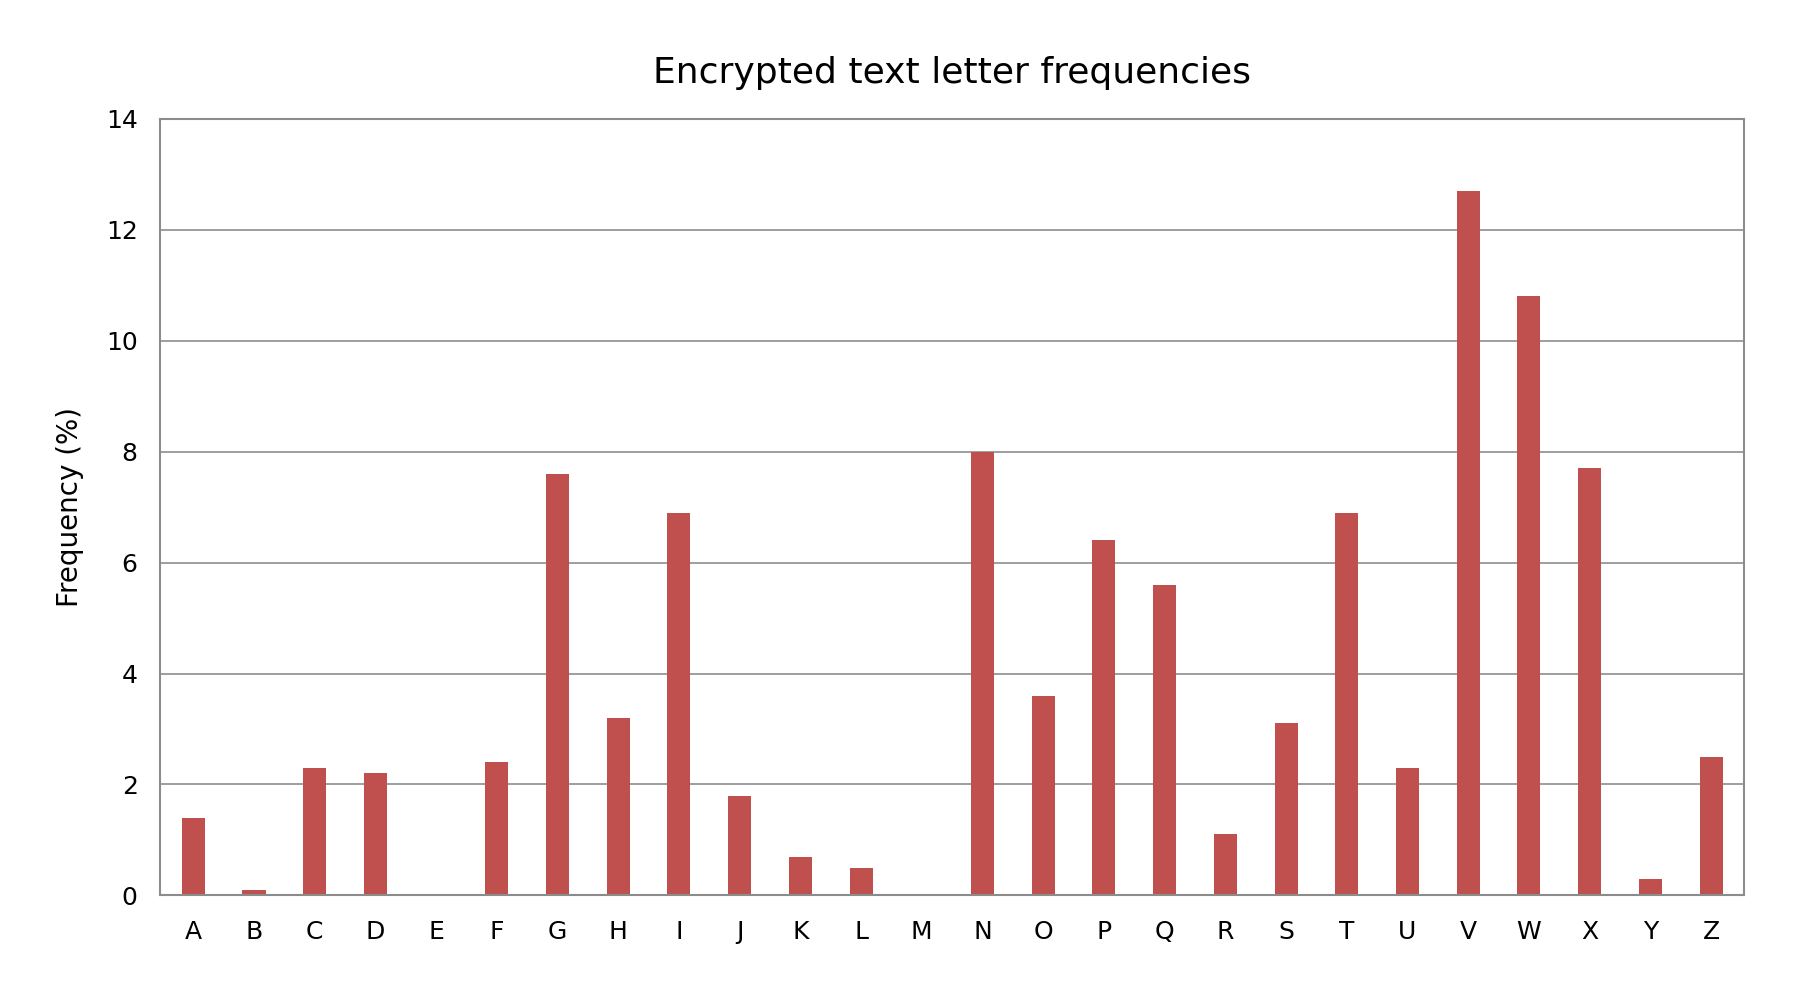
\includegraphics[width=0.94\linewidth]{screenshots/encrypted_frequency_percentages.png}
\captionof{figure}{Ciphertext profile: the highest peaks occur at V and W}
\label{fig:cipher-chart}
\end{center}

The cipher relabels the letters of this particular passage; it does not force the passage to have exactly the average English distribution. Similar peaks suggest initial matches, while word evidence determines whether they are correct. The following reconstruction preserves that distinction between a statistical guess and a substitution supported by readable context.


\clearpage
\section{Step-by-step recovery of the substitution}
\label{sec:deductions}
The following sequence follows the 19 steps recorded during the exercise. The first decisions use frequency; later decisions rely increasingly on words revealed by earlier replacements. A candidate was useful when it explained several occurrences without contradicting the existing mapping.

\subsection{Steps 1--7: establishing common letters}
\begin{enumerate}
\item \textbf{\mapto{V}{e}: the strongest frequency match.} Ciphertext \texttt{V} has 327 occurrences, approximately 12.74\% of all letters, and is the most frequent symbol. This closely matches the English reference for \texttt{e}, making it the initial hypothesis.

\item \textbf{\mapto{W}{t}: the second major peak.} Ciphertext \texttt{W} occurs 276 times, approximately 10.75\%. Its high rank suggests \texttt{t}, even though this passage contains more of it than the average English percentage. Together, the first two replacements expose many occurrences of \texttt{tQe}.

\item \textbf{\mapto{Q}{h}: recognizing \texttt{the}.} The repeated trigraph \texttt{tQe} is naturally read as \texttt{the}. This yields \texttt{h} and supplies word-level support for the earlier choices of \texttt{t} and \texttt{e}.

\item \textbf{\mapto{T}{a}: recognizing \texttt{that}.} The pattern \texttt{thTt} becomes \texttt{that}. Ciphertext \texttt{T} also occurs as a one-letter word, supporting \texttt{a}. The agreement between a word pattern and a grammatical clue is stronger than a frequency guess alone.

\item \textbf{\mapto{P}{s}: recognizing \texttt{these}.} The pattern \texttt{thePe} suggests \texttt{these}. Ciphertext \texttt{P} occurs 165 times, approximately 6.43\%, close to the English reference of 6.33\% for \texttt{s}. The screenshot rounds the observed value to 6.4\%.

\item \textbf{\mapto{N}{o}: recognizing \texttt{to}.} The frequent two-letter pattern \texttt{tN} becomes \texttt{to}. The observed 205 occurrences, approximately 7.99\%, are compatible with a common vowel. This decision demonstrates why frequency ranks must be checked against words: \texttt{N} is third in the ciphertext ranking but represents \texttt{o}, not \texttt{a}.

\item \textbf{\mapto{X}{i}: recognizing \texttt{it}.} The pattern \texttt{Xt} is read as \texttt{it}. The observed frequency, 198 occurrences or approximately 7.71\%, supports a common letter such as \texttt{i}. This also begins to reveal recurring short grammatical words elsewhere in the passage.
\end{enumerate}

\subsection{Steps 8--12: recovering phrases}
\begin{enumerate}[resume]
\item \textbf{\mapto{Z}{m}, \mapto{I}{r}, \mapto{G}{n}: a complete phrase.} The fragment \texttt{the saZe IeasoG as} becomes \texttt{the same reason as}. It supplies three mutually compatible replacements. Their frequencies remain plausible, but the readable phrase is the decisive evidence. The beginning of the message now contains \texttt{on a} and \texttt{nearSF}.

\item \textbf{\mapto{O}{d}: matching both ends of a phrase.} The fragment \texttt{Oesire to reaO} becomes \texttt{desire to read}. The same unknown symbol occurs at the start of one word and the end of another; both positions support the same letter.

\item \textbf{\mapto{F}{y}, \mapto{S}{l}, \mapto{J}{g}: the opening sentence.} The fragment \texttt{on a daF nearSF 4,000 Fears aJo} becomes ``on a day nearly 4,000 years ago''. The repeated \texttt{F} is explained consistently in \texttt{day}, \texttt{nearly}, and \texttt{years}. This step establishes \texttt{g}, which also resolves endings such as \texttt{doing} and \texttt{writing}.

\item \textbf{\mapto{R}{w}, \mapto{H}{c}: recognizing \texttt{town called}.} The phrase \texttt{in a toRn Halled menet} becomes \texttt{in a town called menet}. The ordinary words provide the evidence; identifying the proper name \texttt{menet} in advance is unnecessary.

\item \textbf{\mapto{C}{f}: \texttt{of} and \texttt{life}.} The fragment \texttt{story oC his lord's liCe} becomes \texttt{story of his lord's life}. The same substitution solves a common preposition and a contextually appropriate noun, strengthening the consistency of the partial key.
\end{enumerate}

\subsection{Steps 13--19: resolving the remaining observed symbols}
\begin{enumerate}[resume]
\item \textbf{\mapto{L}{k}: recognizing \texttt{knows}.} The fragment \texttt{world Lnows it} becomes \texttt{world knows it}. This resolves an uncommon letter using a familiar phrase rather than its low frequency alone.

\item \textbf{\mapto{D}{u}, \mapto{A}{b}: recognizing \texttt{scribe} and \texttt{out}.} The fragment \texttt{a master scriAe sketched oDt} becomes \texttt{a master scribe sketched out}. The replacements also clarify words and names elsewhere, including \texttt{about}, \texttt{tomb}, and \texttt{Khnumhotep}.

\item \textbf{\mapto{U}{p}: recognizing \texttt{hieroglyphs}.} The joined fragment \texttt{thehieroglyUhs} becomes \texttt{thehieroglyphs}. A word boundary can be restored for reading, giving ``the hieroglyphs'', but the missing space is independent of the substitution itself.

\item \textbf{\mapto{B}{q}: recognizing \texttt{technique}.} The word \texttt{techniBue} becomes \texttt{technique}. Ciphertext \texttt{B} occurs only twice, so context is more informative than a frequency ranking for this rare letter.

\item \textbf{\mapto{K}{v}: recognizing \texttt{even}.} The fragment \texttt{eKen the slightest} becomes \texttt{even the slightest}. The same pair also resolves words such as \texttt{developed} and \texttt{service}.

\item \textbf{\mapto{Y}{x}: recognizing \texttt{text}.} The phrase \texttt{read the teYt} becomes \texttt{read the text}. This provides a clear context for a relatively rare letter: ciphertext \texttt{Y} appears eight times.

\item \textbf{\mapto{E}{j}: recognizing \texttt{just}.} The fragment \texttt{instead of Eust writing} becomes \texttt{instead of just writing}. Ciphertext \texttt{E} appears only once. This final contextual deduction resolves the last symbol actually present in the cryptogram.
\end{enumerate}

\clearpage
\section{Progressive decryption}
\label{sec:progress}
Each sample shows the same opening three lines, so the effect of accumulating substitutions can be compared directly. Uppercase characters are unresolved ciphertext; lowercase characters are recovered plaintext. Line wrapping is adjusted for page width. The grouping follows the supplied progress record. The full 19-step sequence is explained in Section~\ref{sec:deductions}.

\subsection{After steps 1 and 2}
Only \mapto{V}{e} and \mapto{W}{t} are known. The repeated pattern \texttt{tQe} becomes visible.
\sample{stage-02.txt}

\subsection{After step 3}
The substitution \mapto{Q}{h} resolves \texttt{the}, giving a reliable anchor at several locations.
\sample{stage-03.txt}

\subsection{After step 4}
The substitution \mapto{T}{a} reveals the one-letter word \texttt{a} and the word \texttt{that}.
\sample{stage-04.txt}

\subsection{After steps 5 and 6}
The additional pairs \mapto{P}{s} and \mapto{N}{o} reveal common word fragments and make the sentence structure easier to follow.
\sample{stage-06.txt}

\subsection{After steps 7 and 8}
Adding \texttt{i}, \texttt{m}, \texttt{r}, and \texttt{n} makes \texttt{on a}, \texttt{master}, and \texttt{his} readable. The broader passage supplies the phrase \texttt{the same reason as} used in step 8.
\sample{stage-08.txt}

\subsection{After steps 9 and 10}
The opening now reads ``on a day nearly 4,000 years ago''. The new substitutions also reveal words such as \texttt{nile} and \texttt{story}.
\sample{stage-10.txt}

\subsection{After steps 11 and 12}
The substitutions for \texttt{w}, \texttt{c}, and \texttt{f} expose ``in a town called'' and ``story of his lord's life''.
\sample{stage-12.txt}

\subsection{After steps 13--15}
The remaining letters in \texttt{scribe}, \texttt{sketched}, and \texttt{hieroglyphs} are resolved. The opening sample happens to contain none of the symbols still awaiting steps 16--19; the rest of the passage still needs them.
\sample{stage-15.txt}

\subsection{After steps 16--19}
The whole ciphertext is now readable. This opening sample is unchanged from the preceding one because the final four pairs are established elsewhere, in \texttt{technique}, \texttt{even}, \texttt{text}, and \texttt{just}.
\sample{stage-19.txt}

These samples illustrate why a short readable excerpt is not sufficient proof that the entire message has been solved. The final verification must cover every symbol and the complete passage.

\clearpage
\section{Recovered key and final result}
\subsection{The recovered substitution alphabet}
Table~\ref{tab:key} records the direction used throughout the solution: ciphertext letters map to plaintext letters. The 19 steps identify 25 pairs because some steps establish several pairs at once.

\begin{table}[htbp]
\centering
\caption{Ciphertext-to-plaintext substitution key}
\label{tab:key}
\small
\begin{tabular}{c*{13}{c}}
\hline
Ciphertext & A & B & C & D & E & F & G & H & I & J & K & L & M\\
Plaintext & b & q & f & u & j & y & n & c & r & g & v & k & z*\\
\hline
Ciphertext & N & O & P & Q & R & S & T & U & V & W & X & Y & Z\\
Plaintext & o & d & s & h & w & l & a & p & e & t & i & x & m\\
\hline
\end{tabular}
\par\smallskip\footnotesize *The pair \mapto{M}{z} is inferred by elimination; ciphertext M does not occur.
\end{table}

All 25 observed ciphertext letters have distinct plaintext values. The only unused plaintext letter is \texttt{z}; therefore, assuming a permutation of the full 26-letter alphabet, the remaining pair must be \mapto{M}{z}. No occurrence in this passage directly tests that pair.

\subsection{Verification of the result}
The recovered mapping explains the full passage consistently, including the common words used to derive it and the less common names that emerged later. It also preserves the expected repeated-letter structures. For example, a doubled ciphertext symbol must decrypt to a doubled plaintext letter, rather than requiring a different interpretation in each position.

As a preparation check, the inverse mapping was applied to the literal decrypted text. It reproduced the supplied ciphertext exactly after case normalization, including its punctuation, spacing, and line breaks. This confirms consistent application of the recovered key; by itself, a round trip would not prove that a guessed key gives the intended English message. Here the readable text and the independent word clues provide that additional evidence. The 26 integer frequency counts also match the screenshot exactly, including the zero count for \texttt{M}.

\subsection{Complete plaintext: reading version}
\label{sec:plaintext}
The following version applies the recovered key and restores obvious missing word boundaries and sentence capitalization. Paragraph breaks are editorial. The stray bullet before \texttt{proliferated} is omitted. No letter sequence is changed relative to the literal decryption apart from capitalization; the original joined words remain available in Appendix~\ref{app:literal}. The historical statements are part of the recovered passage, not separate findings established by this cryptanalysis exercise.

\begin{quote}
On a day nearly 4,000 years ago, in a town called Menet Khufu bordering the thin ribbon of the Nile, a master scribe sketched out the hieroglyphs that told the story of his lord's life—and in so doing he opened the recorded history of cryptology. His was not a system of secret writing as the modern world knows it; he used no fully developed code of hieroglyphic symbol substitutions. His inscription, carved about 1900 B.C. into the living rock in the main chamber of the tomb of the nobleman Khnumhotep II, merely uses some unusual hieroglyphic symbols here and there in place of the more ordinary ones. Most occur in the last 20 columns of the inscription's 222, in a section recording the monuments that Khnumhotep had erected in the service of the pharaoh Amenemhet II.

The intention was not to make it hard to read the text. It was to impart a dignity and authority to it, perhaps in the same way that a government proclamation will spell out ``In the year of Our Lord One thousand eight hundred and sixty three'' instead of just writing ``1863.'' The anonymous scribe may also have been demonstrating his knowledge for posterity. Thus the inscription was not secret writing, but it incorporated one of the essential elements of cryptography: a deliberate transformation of the writing. It is the oldest text known to do so.

The transformations occur in funerary formulas, in a hymn to Thoth, in a chapter of the Book of the Dead, on the sarcophagus of the pharaoh Seti I, in royal titles displayed in Luxor, on the architrave of the Temple of Luxor, on stele, in laudatory biographic inscriptions. There is nothing meant to be concealed in all this; indeed, many of the statements are repeated in ordinary form right next to the altered ones. Why, then, the transformations? Sometimes for essentially the same reason as in Khnumhotep's tomb: to impress the reader. Occasionally for a calligraphic or decorative effect; rarely, to indicate a contemporary pronunciation; perhaps even for a deliberate archaism as a reaction against foreign influence.

But many inscriptions are tinctured, for the first time, with the second essential for cryptology—secrecy. In a few cases, the secrecy was intended to increase the mystery and hence the arcane magical powers of certain religious texts. But the secrecy in many more cases resulted from the understandable desire of the Egyptians to have passersby read their epitaphs and so confer upon the departed the blessings written therein.

In Egypt, with its concentration upon the afterlife, the number of these inscriptions soon proliferated to such an extent that the attention and the goodwill of visitors flagged. To revive their interest, the scribes deliberately made the inscriptions a bit obscure. They introduced the cryptographic signs to catch the reader's eye, make him wonder, and tempt him into unriddling them—and so into reading the blessings. It was a sort of Madison Avenue technique in the Valley of the Kings. But the technique failed utterly. Instead of interesting the readers, it evidently destroyed even the slightest desire to read the epitaphs, for soon after the funerary cryptography was begun, it was abandoned.
\end{quote}


\clearpage
\section{Conclusions}
The laboratory demonstrated how an English monoalphabetic substitution can be recovered without exhaustive key search. Frequencies suggested the initial \texttt{e} and \texttt{t} replacements; common patterns such as \texttt{the}, \texttt{that}, and \texttt{to} then constrained the solution. As the passage became readable, longer phrases and specific words resolved the rarer letters.

The 19 recorded steps recovered all 25 symbols present in the 2,567-letter cryptogram. The remaining alphabet pair was inferred by elimination and explicitly distinguished from observed evidence. Each recovered pair was applied consistently throughout the passage.

The central lesson is that frequency analysis is a starting point, not an automatic letter-ranking substitution. Statistical clues become convincing when supported by grammar, word shapes, and repeated occurrences. A large nominal key space does not protect a cipher that retains so much language structure. The exercise also connects with Laboratory Work No. 1: permuting an alphabet may enlarge the key space, but a fixed monoalphabetic substitution still preserves frequencies.

\section*{Report materials}
\addcontentsline{toc}{section}{Report materials}
This laboratory required no application source code. Its materials consist of the ciphertext, recovered key, progress samples, screenshots, and this report, kept under \texttt{Lab\_2} in the laboratory repository:
\begin{center}\url{\repositoryurl}\end{center}

\clearpage
\begin{thebibliography}{9}
\addcontentsline{toc}{section}{References}
\bibitem{handout} \textit{Laboratory Work No. 2: Cryptanalysis of Monoalphabetic Ciphers}. Supplied course material, Sections 2.1--2.2. Theory and reference frequencies translated from Romanian for this report.
\bibitem{tool} Daniel Rodriguez-Clark, Crypto Corner. \textit{Frequency Analysis: Breaking the Code}. Interactive activity used for the laboratory. Accessed 9 October 2026.\\
\url{https://crypto.interactive-maths.com/frequency-analysis-breaking-the-code.html}
\bibitem{records} Gabriel Balan. \textit{Laboratory Work No. 2 working records}. Supplied ciphertext, four frequency screenshots, ordered substitution notes, and intermediate plaintext extracts.
\end{thebibliography}

\clearpage
\appendix
\section{Complete supplied ciphertext}
\label{app:ciphertext}
The following transcription preserves the supplied letters, punctuation, line breaks, and missing spaces. Backslashes used to mark line breaks in the pasted message are formatting markers and are not part of the cryptogram. Case is ignored during frequency counting and substitution.
{\VerbatimInput[fontsize=\fontsize{8.5}{10}\selectfont]{data/ciphertext.txt}}

\clearpage
\section{Literal decrypted text}
\label{app:literal}
This is the direct character-for-character result of the recovered mapping, with plaintext letters in lowercase. Unlike the reading version in Section~\ref{sec:plaintext}, it retains joined words, original line breaks, and the stray bullet. It provides an exact basis for re-encryption after ignoring ciphertext case.
{\VerbatimInput[fontsize=\fontsize{8.5}{10}\selectfont]{data/plaintext-literal.txt}}
\end{document}
